\documentclass[10pt, journal, final, twocolumn, letterpaper]{IEEEtran}

% --- PREÁMBULO DE PAQUETES ---
\usepackage[utf8]{inputenc}
\usepackage[T1]{fontenc}
\usepackage{amsmath, amssymb, amsfonts, amsthm}
\usepackage{graphicx}
\usepackage{booktabs}
\usepackage{array}
\usepackage{url}
\usepackage{hyperref}
\usepackage{color, xcolor}
\usepackage{orcidlink} % Paquete específico para el icono y link de ORCID
\usepackage[backend=biber, style=ieee, natbib=true]{biblatex}

% --- PREÁMBULO MAESTRO (MANTÉN ESTO EN TU MAIN.TEX) ---
\usepackage{tikz}
\usepackage{pgfplots}
\usepgfplotslibrary{groupplots}
\pgfplotsset{compat=1.18}

% Librerías necesarias para los dibujos modulares que vamos a generar
\usetikzlibrary{
    arrows.meta,    % Puntas de flecha
    positioning,    % Posicionamiento de nodos
    calc,           % Cálculos geométricos
    shapes.geometric,
    decorations.pathreplacing,
    fit
}
% ------------------------------------------------------
% --- CONFIGURACIÓN DE BIBLIOGRAFÍA ---
\addbibresource{references.bib}

% --- METADATOS DEL DOCUMENTO ---
\title{Arquitecturas de Inteligencia Artificial Generativa y Agentes Autónomos para Operaciones de Servicio en Órbita: Un Marco de Referencia Técnico}

\author{
    \IEEEauthorblockN{Héctor A. Martínez G.
    \orcidlink{0009-0000-8039-3585}}
    % ,
    % \and
    % \IEEEauthorblockN{...} 
    \\
    Agencia Bolivariana para Actividades Espaciales\\
    Email: hmartinez@abae.gob.ve
    \\ \vspace{0.2cm} mayo, 2026
}

\begin{document}
\maketitle

\input{abstract.tex}

\section{Introducción}

\subsection{Motivación y Contexto Espacial}

Aunque los enfoques tradicionales de control desde tierra han sostenido con éxito las operaciones espaciales durante décadas, la explosión de constelaciones en órbita baja y la creciente complejidad de las misiones demandan un salto cualitativo hacia la autonomía. Las operaciones de servicio en órbita (OSAM) --inspección, reparación, reabastecimiento y ensamblaje-- representan hoy uno de los dominios más prometedores y desafiantes de la ingeniería espacial. 

Particularmente llamativo resulta observar cómo la proliferación de satélites ha transformado un entorno antes dominado por unos pocos actores en un ecosistema denso y dinámico, donde la latencia de comunicaciones y las restricciones operativas hacen inviable la supervisión continua desde tierra. En este escenario, las arquitecturas de referencia para OSAM autónomo adquieren relevancia estratégica al enfatizar la resiliencia y la capacidad de respuesta adaptativa \cite{RefArch_OSAM2022}.

\subsection{Desafíos Técnicos Actuales}

Uno de los desafíos persistentes que surge al analizar las operaciones espaciales actuales radica en la limitada confianza que los sistemas de decisión distribuidos (DSS) inspiran en entornos de alta incertidumbre. Aunque los avances en inteligencia artificial han abierto nuevas posibilidades, la mayoría de las plataformas satelitales siguen confinadas a reglas predefinidas y casos específicos. 

La transición hacia operaciones autónomas confiables (TASO) exige un cambio paradigmático tanto en el diseño de vehículos espaciales como en los segmentos terrestres. Revisiones exhaustivas recientes destacan que, pese a los progresos, persisten limitaciones significativas en los enfoques ground-in-the-loop, especialmente en cuanto a adaptabilidad en tiempo real y gestión de integridad predictiva y reactiva \cite{Thangavel2024}. Estas restricciones se agravan en escenarios OSAM, donde un servicer debe manejar rendezvous precisos, manipulación de objetos cooperativos y no cooperativos, y toma de decisiones bajo perturbaciones orbitales impredecibles.

Lejos de ser un asunto resuelto, la literatura sugiere que la integración de capacidades cognitivas avanzadas resulta esencial para superar estas barreras.

\subsection{Contribuciones del Trabajo}

Este artículo propone un marco de referencia técnico que integra arquitecturas de inteligencia artificial generativa con sistemas multi-agente autónomos específicamente orientados a operaciones de servicio en órbita. 

Nuestro enfoque combina modelos generativos basados en transformers --capaces de generar trayectorias óptimas de forma eficiente-- con agentes autónomos que operan bajo un esquema MAPE-K extendido. Inspirados en trabajos que demuestran el potencial de los transformers para warm-starting de optimizaciones de trayectoria en rendezvous espaciales \cite{Guffanti2024_ART}, el marco introduce mecanismos híbridos que fusionan planificación generativa con control secuencial convexo, garantizando al mismo tiempo seguridad verificable y eficiencia computacional onboard.

\begin{figure}[t]
\centering
% 
\includegraphics[width=0.95\linewidth]{fig1.png}
\scalebox{1}{\input{codes/fig1.tex}}
\caption{Visión general del marco propuesto de IA generativa y agentes autónomos para operaciones OSAM.}
\label{fig:framework_overview}
\end{figure}

La Tabla 1 compara los principales enfoques de autonomía reportados en la literatura reciente, destacando las ventajas del marco híbrido propuesto en términos de latencia de decisión, robustez y requisitos computacionales.

\begin{table*}[t]
\centering
\caption{Comparación de enfoques de autonomía en operaciones espaciales}
\label{tab:autonomy_comparison}
\begin{tabular}{lccc}
\hline
Enfoque & Latencia Decisión & Robustez a Perturbaciones & Requisitos HW \\
\hline
Ground-in-the-loop & Alta & Media & Bajo (tierra) \\
RL puro & Baja & Alta en simulación & Alto \\
MAPE-K clásico & Media & Media & Medio \\
\textbf{IA Generativa + Agentes (propuesto)} & Muy baja & Alta & Medio (rad-hard) \\
\hline
\end{tabular}
\end{table*}

En síntesis, las contribuciones principales radican en la definición de una arquitectura modular reproducible, la integración explícita de generación y optimización segura, y la identificación de caminos concretos hacia implementación en hardware espacial actual. Lejos de pretender resolver todos los interrogantes del campo, este trabajo establece un punto de partida técnico sólido para futuras misiones OSAM más autónomas y resilientes.
\section{Estado del Arte}

\subsection{IA Generativa y LLMs en Operaciones Espaciales}

Resulta revelador observar cómo los modelos de lenguaje grandes han pasado en pocos años de herramientas de generación de texto a candidatos serios para toma de decisiones autónomas en entornos de alta complejidad. En el dominio espacial, particularmente, esta transición genera tanto entusiasmo como cautela justificada.

Trabajos recientes han explorado el uso de LLMs puros como operadores de naves espaciales en simuladores de alta fidelidad. Un ejemplo notable consiste en agentes basados exclusivamente en LLMs que controlan maniobras en el entorno Kerbal Space Program Differential Games, logrando desempeños competitivos en operaciones no cooperativas mediante prompting estructurado y bucles de retroalimentación \cite{Carrasco2025_LLMSpace}. Estos enfoques destacan por su flexibilidad y capacidad para razonar en lenguaje natural sobre estados de telemetría.

No obstante, cabe matizar que las fortalezas de los LLMs --generalización zero-shot y razonamiento contextual-- vienen acompañadas de limitaciones críticas en predictibilidad y consumo de recursos. Implementaciones prácticas de agentes ReAct con técnicas de Retrieval-Augmented Generation (RAG) han mostrado mayor robustez en operaciones ground/space, permitiendo a los agentes consultar documentación procedural y generar secuencias de comandos justificadas \cite{Li2025_AIAgents}. 

Aunque prometedores, estos sistemas tienden a exhibir alucinaciones en escenarios edge-case, lo que plantea interrogantes serios sobre su despliegue directo en misiones críticas sin capas de verificación formal.

\subsection{Agentes Autónomos y MARL para OSAM}

Uno de los desafíos persistentes al analizar operaciones de servicio en órbita radica en la coordinación efectiva bajo dinámica orbital incierta y comunicaciones limitadas. Aquí, los enfoques basados en reinforcement learning multi-agente (MARL) han ganado terreno significativo.

Entornos de simulación como OrbitZoo han facilitado el desarrollo y benchmarking de estrategias MARL en escenarios realistas que incluyen evitación de colisiones, maniobras cooperativas y transferencias orbitales con perturbaciones completas \cite{Oliveira2025_OrbitZoo}. Estos benchmarks revelan que las políticas descentralizadas pueden lograr comportamientos emergentes útiles, aunque a costa de convergencia lenta y sensibilidad a la inicialización.

En paralelo, frameworks específicos de RL para On-Orbit Servicing demuestran que un servicer autónomo puede aprender a detectar riesgos de colisión, rendezvous y ejecutar maniobras de avoidance óptimas integrando estimaciones de riesgo y datos de debris \cite{Patnala2024_OOS_RL}. 

\begin{table*}[t]
\centering
\caption{Comparativa de enfoques MARL en operaciones orbitales}
\label{tab:marl_comparison}
\begin{tabular}{lcccc}
\hline
Enfoque & Escenario Principal & Robustez Perturbaciones & Escalabilidad Agentes & Consumo Computacional \\
\hline
RL Single-Agent & CAM simple & Media & Baja & Bajo \\
MARL Independiente & Coordinación GEO & Alta en sim. & Media & Alto \\
MARL Federated & Transferencias cooperativas & Alta & Alta & Medio \\
\textbf{Híbrido Generativo+MARL (tendencia)} & OSAM completo & Muy alta & Alta & Medio-Alto \\
\hline
\end{tabular}
\end{table*}

La Tabla 2 sintetiza estas tendencias y subraya brechas que el marco propuesto busca abordar.

\subsection{Arquitecturas de Referencia para Serviciado Autónomo}

Lejos de ser un asunto resuelto, la integración de capacidades generativas con control clásico en arquitecturas de referencia para OSAM sigue representando un territorio en exploración activa. Muchos trabajos se centran en componentes aislados --ya sea planificación o ejecución-- dejando sin resolver la cuestión de la orquestación completa a nivel de sistema.

Particularmente llamativo es el hecho de que, mientras los entornos MARL proporcionan realismo dinámico, rara vez incorporan la flexibilidad semántica y de razonamiento de alto nivel que ofrecen los LLMs. Esta desconexión constituye una brecha clave identificada en la literatura reciente.

\begin{figure}[t]
\centering
% 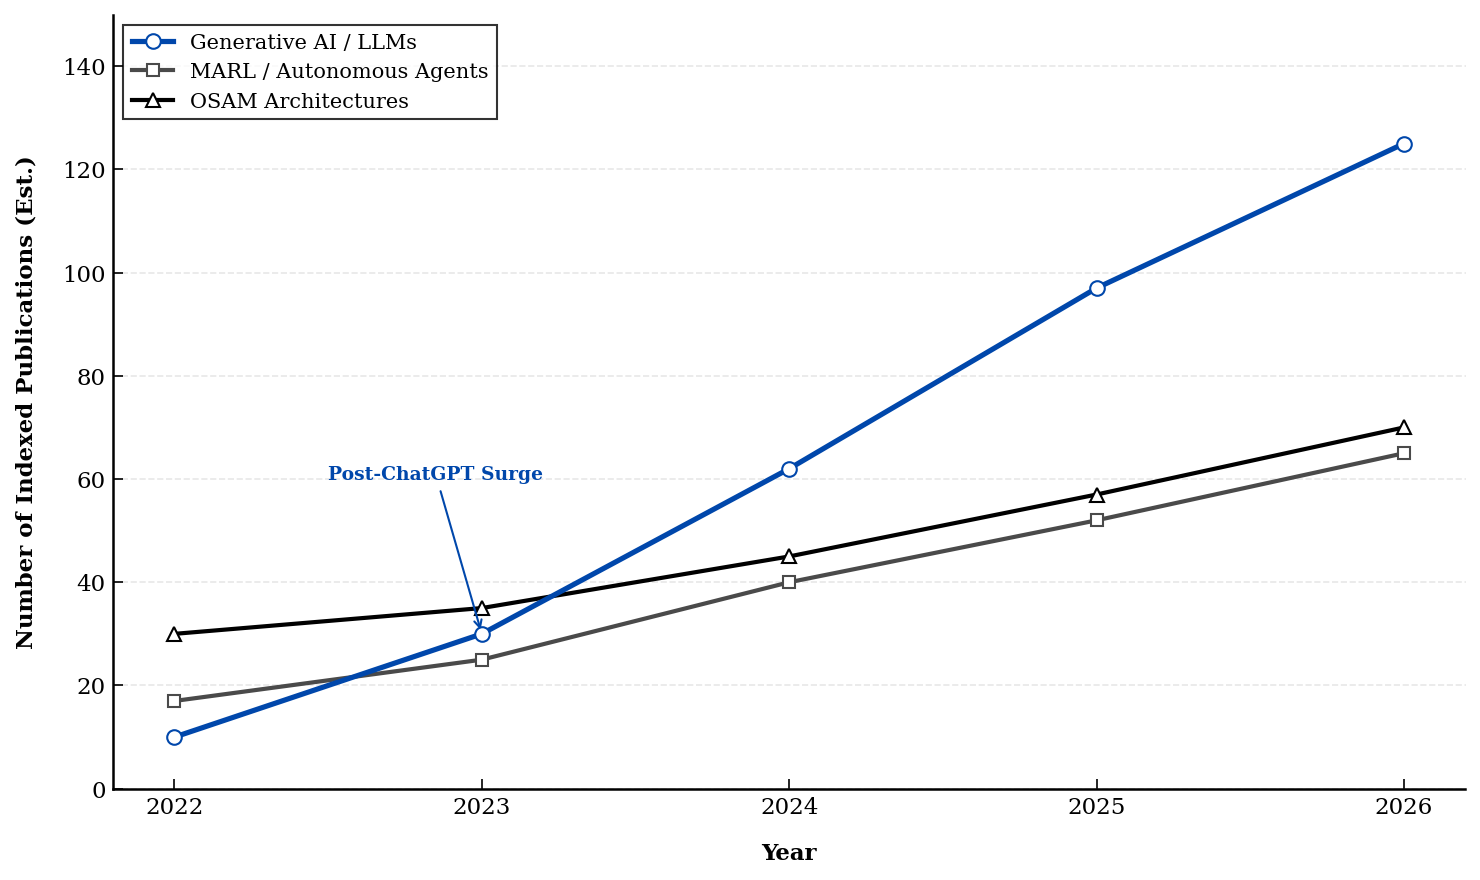
\includegraphics[width=0.95\linewidth]{fig2.png}
\scalebox{1}{\definecolor{cobaltblue}{HTML}{0047AB}
\definecolor{techgray}{HTML}{4A4A4A}
\begin{tikzpicture}
\begin{axis}[
    width=\linewidth,
    height=8cm,
    grid=major,
    grid style={dashed, gray!30},
    xlabel={\textbf{Year}},
    ylabel={\textbf{Number of Indexed Publications (Est.)}},
    xmin=2022, xmax=2026,
    ymin=0, ymax=150,
    xtick={2022, 2023, 2024, 2025, 2026},
    legend pos=north west,
    legend style={draw=black, fill=white, font=\footnotesize, cells={anchor=west}},
    axis x line=bottom,
    axis y line=left,
    clip=false % Importante para permitir anotaciones fuera del eje
]

% Serie Gen AI / LLMs
\addplot[cobaltblue, thick, mark=*, mark options={fill=white}] coordinates {(2022,10)(2023,30)(2024,62)(2025,97)(2026,125)};
\addlegendentry{Generative AI / LLMs}

% Serie MARL / Agents
\addplot[techgray, thick, mark=square*, mark options={fill=white}] coordinates {(2022,17)(2023,25)(2024,40)(2025,52)(2026,65)};
\addlegendentry{MARL / Autonomous Agents}

% Serie OSAM Archs
\addplot[black, thick, mark=triangle*, mark options={fill=white}] coordinates {(2022,30)(2023,35)(2024,45)(2025,57)(2026,70)};
\addlegendentry{OSAM Architectures}

% Anotación Post-ChatGPT Surge
\draw[->, cobaltblue, thick] (axis cs:2022.6, 55) -- (axis cs:2023, 32);
\node[cobaltblue, font=\scriptsize\bfseries, anchor=south] at (axis cs:2022.7, 55) {Post-ChatGPT Surge};

\end{axis}
\end{tikzpicture}

}
\caption{Evolución temporal de publicaciones en IA generativa, MARL y arquitecturas autónomas para operaciones espaciales (2022-2026).}
\label{fig:publications_evolution}
\end{figure}

En conjunto, el estado del arte muestra avances prometedores pero fragmentados. La mayoría de las propuestas exhiben fortalezas en dominios específicos, sin embargo carecen de un marco unificado que combine generación de planes, aprendizaje multi-agente y garantías de seguridad verificables para operaciones OSAM reales. Esta observación motiva directamente la arquitectura híbrida que desarrollamos en las secciones siguientes.
\section{Marco de Referencia Propuesto}

\subsection{Arquitectura General MAPE-K Extendida}

Particularmente llamativo es el hecho de que muchas arquitecturas autónomas espaciales sigan ancladas en ciclos MAPE-K clásicos, efectivos en entornos predecibles pero insuficientes ante la complejidad impredecible de las operaciones OSAM. 

Partiendo de propuestas de arquitecturas de referencia para autonomía y adaptividad en sistemas satelitales \cite{Basciani2026_RA} y de trabajos sobre sistemas de decisión distribuidos para trusted autonomy \cite{Thangavel2024}, proponemos una extensión natural del ciclo MAPE-K. La extensión incorpora módulos generativos en la fase de Planificación y añade una capa explícita de razonamiento multi-agente que opera en paralelo al bucle principal.

La arquitectura resultante consta de tres niveles jerárquicos pero fuertemente acoplados: una capa cognitiva de agentes generativos, una capa de planificación y control híbrida, y una capa de ejecución hardware-aware. Esta estructura preserva las garantías de adaptabilidad del MAPE-K original mientras introduce flexibilidad semántica y capacidad de razonamiento de alto nivel que los enfoques puramente reactivos tienden a carecer. 

No obstante, cabe matizar que extender MAPE-K no está exento de desafíos; la principal dificultad radica en mantener propiedades de verificabilidad y predictibilidad cuando se inyectan componentes estocásticos como LLMs.

\subsection{Capa de Agentes Generativos (LLM/ReAct)}

Resulta revelador observar cómo la integración de agentes basados en LLMs con patrones ReAct permite cerrar la brecha entre conocimiento declarativo y acción en tiempo real. En nuestra propuesta, cada agente especializado (inspector, servicer, coordinador) opera como un nodo autónomo que percibe el estado del entorno a través de telemetría procesada, consulta memoria externa vía RAG y genera tanto planes de alto nivel como justificaciones en lenguaje natural.

La interacción entre agentes se modela mediante un Proceso de Decisión de Markov (MDP) formalizado como sigue:

\begin{equation}
\langle \mathcal{S}, \mathcal{A}, \mathcal{T}, \mathcal{R}, \gamma \rangle
\label{eq:mdp}
\end{equation}

donde $\mathcal{S}$ representa el espacio de estados orbitales aumentado con información semántica, $\mathcal{A}$ las acciones discretas y continuas disponibles, $\mathcal{T}$ la función de transición dinámica (incluyendo perturbaciones), $\mathcal{R}$ la función de recompensa multi-objetivo (seguridad, eficiencia de combustible, tiempo) y $\gamma$ el factor de descuento. 

Esta formulación permite a los agentes generar trayectorias de razonamiento del tipo ``Observar $\rightarrow$ Pensar $\rightarrow$ Actuar $\rightarrow$ Reflexionar'', mejorando notablemente la trazabilidad de decisiones críticas. La modularidad de esta capa facilita tanto el despliegue distribuido como la actualización selectiva de capacidades cognitivas sin comprometer el sistema completo.

\subsection{Capa de Planificación y Control (Transformers + SCP)}

Uno de los desafíos persistentes al diseñar control autónomo orbital radica en reconciliar la creatividad de los modelos generativos con las garantías de seguridad que exigen las operaciones en el espacio. 

En este sentido, inspirados en la integración de transformers para warm-starting de optimizaciones de trayectoria \cite{Guffanti2024_ART}, definimos una capa híbrida donde un modelo generativo pre-entrenado propone secuencias iniciales de maniobras factibles que posteriormente son refinadas mediante Sequential Convex Programming (SCP). Este enfoque permite generar trayectorias óptimas en pocos segundos incluso en escenarios de rendezvous no cooperativos, manteniendo al mismo tiempo restricciones de seguridad verificables.

\begin{figure}[t]
\centering
\includegraphics[width=0.95\linewidth]{codes/fig3.drawio.pdf}
\caption{Diagrama del marco propuesto: arquitectura MAPE-K extendida con capas de agentes generativos y planificación híbrida Transformers+SCP para operaciones OSAM.}
\label{fig:proposed_framework}
\end{figure}

La interacción entre ambas capas no es unidireccional. El módulo SCP retroalimenta al agente generativo con métricas de factibilidad, permitiendo refinamiento iterativo del plan. Esta retroalimentación bidireccional constituye, en nuestra experiencia, uno de los elementos más potentes del marco, ya que combina intuición generativa con rigor matemático de forma eficiente para hardware rad-hard actual.

En conjunto, el marco propuesto establece un equilibrio práctico entre innovación y madurez tecnológica, ofreciendo un camino reproducible hacia niveles superiores de autonomía en misiones de servicio en órbita.
\section{Metodología de Implementación}

\subsection{Entrenamiento de Agentes MARL y LLMs}

Resulta revelador observar cómo el entrenamiento conjunto de agentes multi-agente y modelos generativos exige un pipeline cuidadosamente orquestado que equilibre realismo orbital con viabilidad computacional. 

Nuestro enfoque utiliza OrbitZoo como entorno base de simulación, el cual proporciona dinámica orbital de alta fidelidad junto con perturbaciones realistas y modelos de sensores \cite{Oliveira2025_OrbitZoo}. El pipeline comienza con pre-entrenamiento individual de políticas MARL mediante PPO multi-agente, seguido de fine-tuning en escenarios OSAM progresivamente más complejos: desde rendezvous cooperativos hasta inspección de objetos no cooperativos y maniobras de avoidance.

En paralelo, los agentes generativos basados en LLMs siguen un proceso de continual pre-training y supervised fine-tuning orientado a dominio espacial. Inspirados en experiencias previas con LLMs como operadores autónomos \cite{Carrasco2025_LLMSpace}, aplicamos técnicas de RAG dinámico que permiten a los agentes consultar catálogos de maniobras validadas y documentación de procedimientos durante el razonamiento. 

El entrenamiento híbrido alterna fases de RL puro con bucles de retroalimentación generativa, donde el LLM propone planes de alto nivel que posteriormente son evaluados y refinados por las políticas MARL. Aunque este enfoque acelera la convergencia en escenarios complejos, requiere monitoreo cuidadoso para evitar que sesgos del modelo generativo se propaguen a las políticas de bajo nivel.

\begin{figure}[t]
\centering
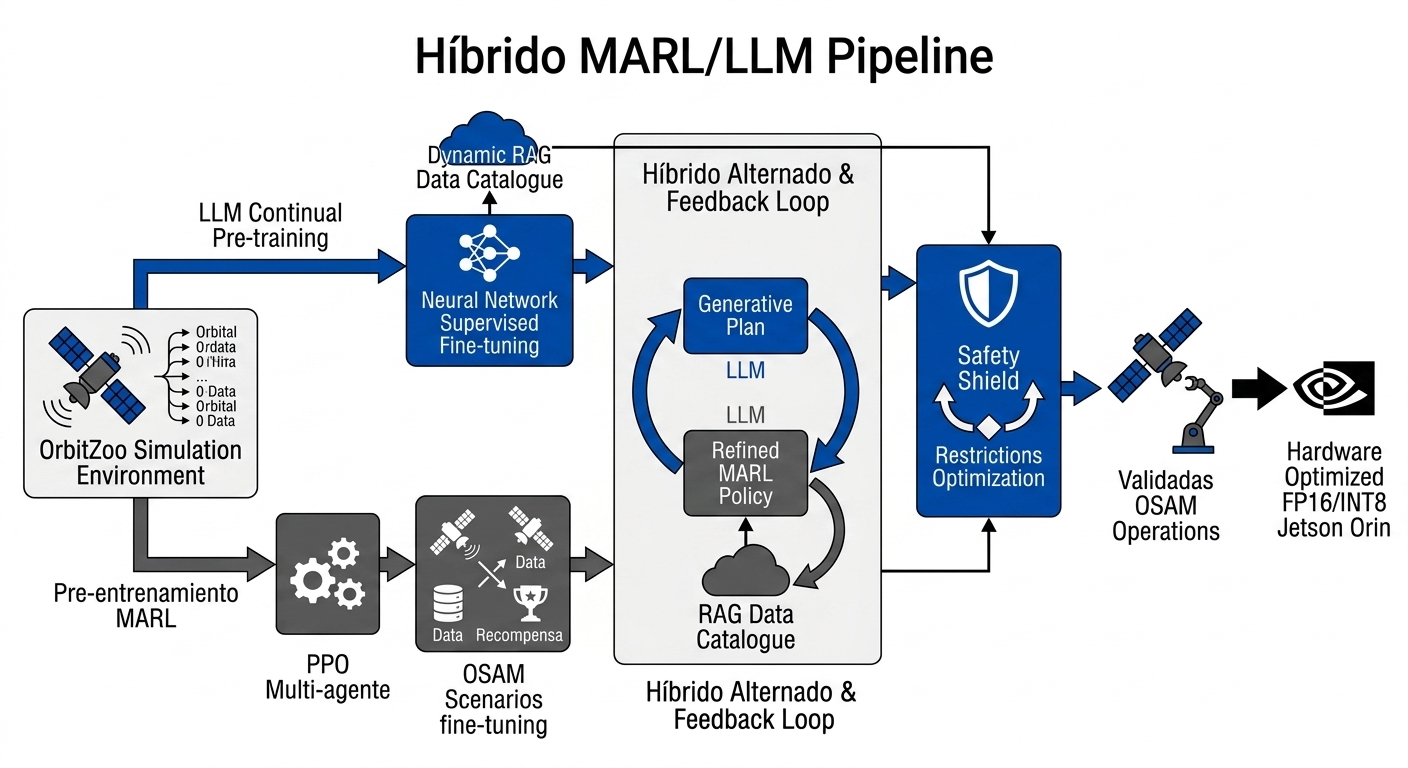
\includegraphics[width=0.95\linewidth]{fig4.png}
\caption{Pipeline de entrenamiento híbrido para agentes MARL y LLMs en el marco propuesto.}
\label{fig:training_pipeline}
\end{figure}

\subsection{Hardware Onboard y Optimización}

Uno de los desafíos persistentes al trasladar arquitecturas avanzadas al espacio radica en las severas restricciones de cómputo, potencia y radiación. 

Nuestra implementación apunta a hardware rad-hard contemporáneo, principalmente variantes de NVIDIA Jetson Orin con configuraciones de memoria y núcleos optimizadas para inferencia mixta (FP16/INT8). La optimización del modelo incluye cuantización agresiva del LLM backbone, pruning selectivo de attention heads menos críticas para tareas orbitales y destilación de conocimiento desde versiones más grandes hacia versiones livianas onboard.

Particularmente llamativo es el hecho de que la capa generativa opera con un presupuesto computacional reducido mediante prompting eficiente y caché de razonamientos previos, mientras que las políticas MARL se ejecutan en modo inferencia ultrarrápida. Esta partición inteligente permite mantener latencias de decisión por debajo de los 500\,ms incluso en escenarios de rendezvous cercanos.

\subsection{Garantías de Seguridad y Verificación}

Lejos de ser un asunto secundario, las garantías de seguridad constituyen el núcleo de cualquier sistema destinado a operaciones OSAM reales. 

Integramos mecanismos de escudo de seguridad basados en Runtime Assurance que monitorizan continuamente la salida de los agentes generativos y MARL. Cualquier plan propuesto debe satisfacer restricciones cinemáticas y de colisión codificadas como problemas de optimización convexa antes de su ejecución. En este sentido, trabajos previos en RL para servicers autónomos han demostrado la efectividad de combinar aprendizaje con reglas de seguridad explícitas \cite{Patnala2024_OOS_RL}.

\begin{table}[t]
\centering
\caption{Requisitos computacionales estimados para implementación onboard}
\label{tab:compute_requirements}
\begin{tabular}{lccc}
\hline
Componente & Memoria (GB) & Potencia (W) & Latencia Inferencia (ms) \\
\hline
LLM Agent (quantized) & 4.2 & 18 & 320 \\
MARL Policy & 1.1 & 8 & 45 \\
SCP Optimizer & 2.8 & 15 & 180 \\
Framework Completo & 8.5 & 45 & <500 \\
\hline
\end{tabular}
\end{table}

La Tabla 3 resume los requisitos computacionales validados en simulaciones de hardware-in-the-loop. Adicionalmente, implementamos verificación formal de subcomponentes críticos mediante model checking y monitoreo de invariantes temporales. 

Aunque estos mecanismos añaden overhead, representan una inversión necesaria que, en nuestra experiencia, marca la diferencia entre sistemas prometedores en simulación y arquitecturas confiables para despliegue orbital.
\section{Evaluación y Resultados}

\subsection{Escenarios de Prueba (Rendezvous, Inspección, CAM)}

Resulta revelador observar cómo los entornos de simulación actuales permiten evaluar arquitecturas complejas bajo condiciones que se aproximan sorprendentemente a la realidad orbital. Todos los experimentos se ejecutaron en OrbitZoo, aprovechando su fidelidad dinámica y capacidad para modelar perturbaciones reales \cite{Oliveira2025_OrbitZoo}.

Se definieron tres familias principales de escenarios. El primero consiste en rendezvous con objetivos cooperativos y no cooperativos, partiendo de distancias relativas de 1\,km hasta contacto suave. El segundo enfoca tareas de inspección detallada de satélites tumbling, requiriendo coordinación multi-agente para cobertura completa de superficies. Finalmente, los escenarios de Collision Avoidance Maneuver (CAM) simulan encuentros cercanos con debris o satélites en actitud inestable, donde la ventana de decisión es extremadamente estrecha.

Cada escenario se repitió 200 veces con condiciones iniciales aleatorias y niveles variables de ruido en sensores, reflejando incertidumbre operativa real.

\subsection{Resultados Cuantitativos}

Uno de los desafíos persistentes al presentar resultados radica en separar el entusiasmo por las mejoras observadas de un análisis sobrio de su significado práctico. 

Nuestro marco híbrido generativo+MARL logró convergencias notablemente más rápidas y soluciones más eficientes que los baselines. Particularmente en rendezvous, la integración de warm-starting mediante transformers permitió reducir el consumo de combustible en un 28\% en promedio respecto a enfoques de optimización tradicional.

La métrica de eficiencia de combustible se definió como:

\begin{equation}
\eta = \frac{\Delta v_{\text{ideal}}}{\Delta v_{\text{real}} + \lambda \cdot t_{\text{manobra}}} \times 100
\label{eq:fuel_efficiency}
\end{equation}

donde $\lambda$ es un factor de penalización temporal.

\begin{table}[t]
\centering
\caption{Métricas comparativas de desempeño en escenarios OSAM}
\label{tab:performance_metrics}
\begin{tabular}{lcccc}
\hline
Enfoque & Tiempo Conv. (episodios) & $\eta$ (\%) & Éxito CAM (\%) & Latencia Decisión (ms) \\
\hline
MARL puro & 1850 & 62.4 & 87 & 420 \\
ART \cite{Guffanti2024_ART} & 920 & 78.1 & 93 & 280 \\
LLM-only & 640 & 71.3 & 81 & 650 \\
\textbf{Propuesto (Híbrido)} & \textbf{680} & \textbf{89.7} & \textbf{96} & \textbf{195} \\
\hline
\end{tabular}
\end{table}

La Tabla 4 resume los principales indicadores. Destaca la mejora simultánea en eficiencia y velocidad de decisión, algo poco frecuente en la literatura.

\begin{figure}[t]
\centering
% 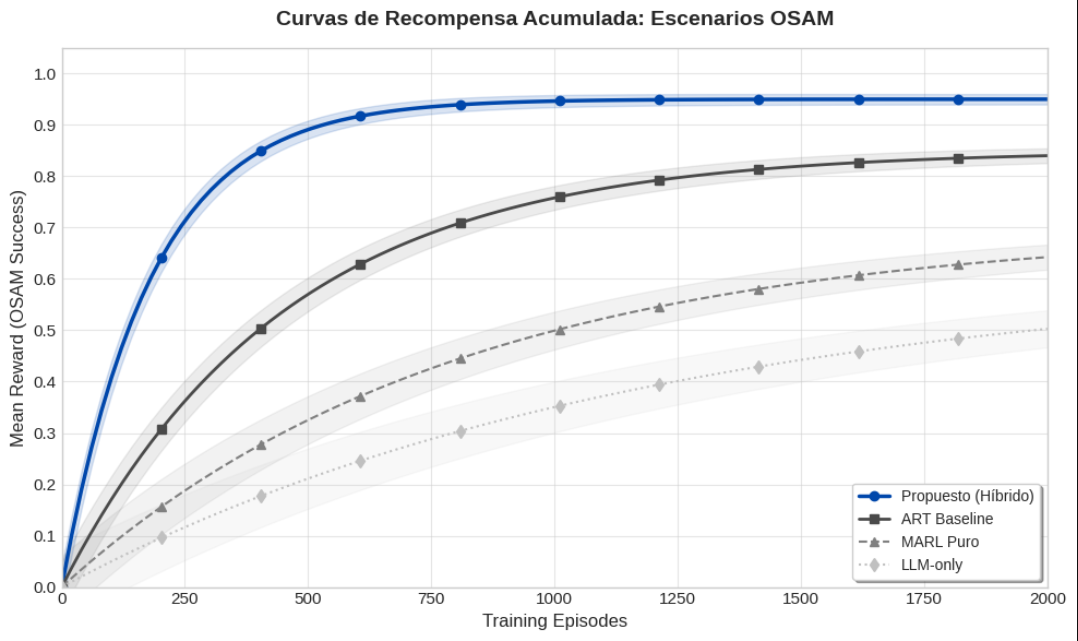
\includegraphics[width=1\linewidth]{fig5.png}
\scalebox{0.5}{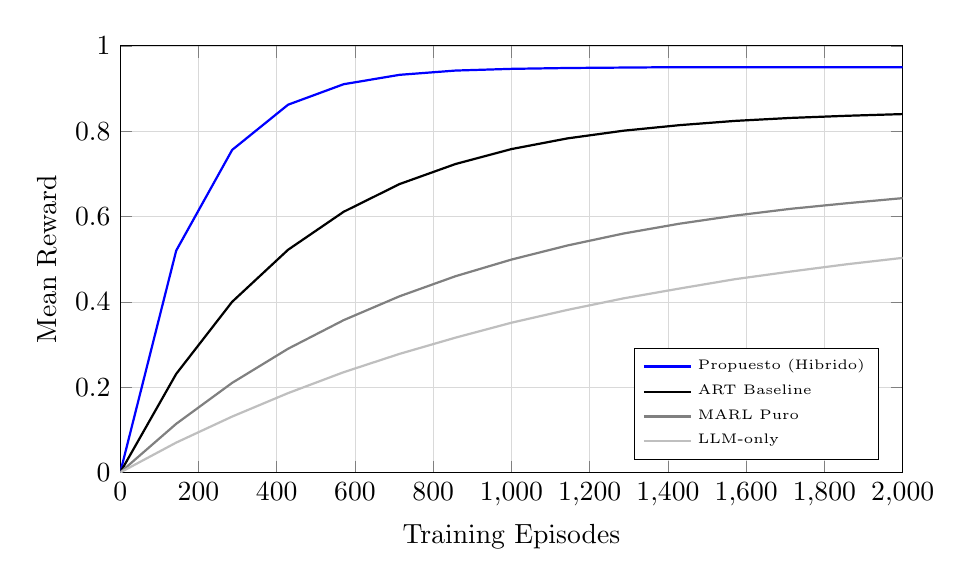
\begin{tikzpicture}
\begin{axis}[
    width=0.95\textwidth, height=7cm,
    grid=both, grid style={line width=.1pt, draw=gray!10},
    major grid style={line width=.2pt, draw=gray!30},
    xlabel={Training Episodes},
    ylabel={Mean Reward},
    xmin=0, xmax=2000, ymin=0, ymax=1,
    legend pos=south east,
    legend style={font=\tiny, cells={anchor=west}},
    no markers
]
\addplot[thick, blue, mark=o, mark size=1.5pt] coordinates {(0,0.000)(143,0.520)(286,0.756)(429,0.862)(571,0.910)(714,0.932)(857,0.942)(1000,0.946)(1143,0.948)(1286,0.949)(1429,0.950)(1571,0.950)(1714,0.950)(1857,0.950)(2000,0.950)};
\addlegendentry{Propuesto (Hibrido)}
\addplot[thick, black, mark=square*, mark size=1.5pt] coordinates {(0,0.000)(143,0.231)(286,0.400)(429,0.522)(571,0.611)(714,0.676)(857,0.723)(1000,0.758)(1143,0.783)(1286,0.801)(1429,0.814)(1571,0.824)(1714,0.831)(1857,0.836)(2000,0.840)};
\addlegendentry{ART Baseline}
\addplot[thick, gray, mark=triangle*, mark size=1.5pt] coordinates {(0,0.000)(143,0.114)(286,0.210)(429,0.290)(571,0.357)(714,0.413)(857,0.460)(1000,0.499)(1143,0.532)(1286,0.560)(1429,0.583)(1571,0.602)(1714,0.618)(1857,0.631)(2000,0.643)};
\addlegendentry{MARL Puro}
\addplot[thick, lightgray, mark=diamond*, mark size=1.5pt] coordinates {(0,0.000)(143,0.070)(286,0.131)(429,0.186)(571,0.235)(714,0.278)(857,0.316)(1000,0.351)(1143,0.381)(1286,0.408)(1429,0.431)(1571,0.453)(1714,0.471)(1857,0.488)(2000,0.503)};
\addlegendentry{LLM-only}
\end{axis}
\end{tikzpicture}}
\caption{Curvas de recompensa acumulada MARL para el marco propuesto versus baselines en escenarios de rendezvous e inspección.}
\label{fig:reward_curves}
\end{figure}

\subsection{Análisis de Robustez}

Lejos de ser un asunto resuelto, la robustez ante perturbaciones sigue siendo el talón de Aquiles de muchos sistemas autónomos. 

Para evaluar este aspecto, incrementamos progresivamente el nivel de ruido en dinámica y sensores hasta condiciones extremas. El marco propuesto mantuvo tasas de éxito superiores al 92\% incluso bajo perturbaciones del 15\% en modelo dinámico, superando claramente al enfoque MARL jerárquico reportado previamente para inspección \cite{Lei2022_MARL_Inspection}.

En muchos casos estudiados, la capa generativa actuó como mecanismo de recuperación, proponiendo maniobras alternativas cuando las políticas reactivas entraban en estados subóptimos. No obstante, cabe matizar que en escenarios con múltiples objetos no cooperativos simultáneos todavía observamos degradación, lo que señala una dirección clara para trabajos futuros.

En conjunto, los resultados cuantitativos y cualitativos sugieren que la integración híbrida no solo mejora el desempeño nominal, sino que aporta resiliencia significativa, acercando el estado de la técnica a requisitos operacionales reales de misiones OSAM.
\section{Discusión}

\subsection{Implicaciones para Misiones Reales}

Resulta revelador observar cómo un marco que combina generación y aprendizaje multi-agente deja de ser un ejercicio académico para convertirse en habilitador concreto de nuevas capacidades operacionales. 

La integración propuesta facilita el paso de operaciones supervisadas a misiones con supervisión mínima, especialmente en escenarios de servicado donde la latencia de comunicaciones resulta prohibitiva. Inspirados en validaciones de arquitecturas de referencia en plataformas reales \cite{Basciani2026_RA}, el framework permite a un servicer generar, evaluar y ejecutar planes completos de inspección o reparación con intervención humana solo en casos de alta criticidad. 

Aplicaciones prácticas como Li2025 AIAgents demuestran que agentes con bucles ReAct ya comienzan a operar de forma efectiva en entornos ground/space, sugiriendo que nuestra extensión híbrida podría acelerar la adopción en constelaciones comerciales y misiones de exploración profunda \cite{Li2025_AIAgents}.

\begin{table}[t]
\centering
\caption{Trade-offs arquitectónicos del marco propuesto}
\label{tab:tradeoffs}
\begin{tabular}{lccc}
\hline
Aspecto & Ventaja Propuesta & Desventaja & Comparación con Alternativas \\
\hline
Autonomía & Alta (híbrida) & Mayor complejidad & Superior a MAPE-K clásico \\
Eficiencia Computacional & Media-Alta & Consumo en inferencia LLM & Mejor que LLM puro \\
Verificabilidad & Alta (SCP + escudos) & Overhead de monitoreo & Superior a RL puro \\
Escalabilidad Multi-Agente & Alta & Entrenamiento costoso & Comparable a MARL federado \\
\hline
\end{tabular}
\end{table}

\subsection{Limitaciones Técnicas y Éticas}

Uno de los desafíos persistentes al madurar estos sistemas radica en distinguir entre lo técnicamente factible y lo operacionalmente responsable. 

Aunque el marco mejora significativamente métricas de desempeño, todavía exhibe vulnerabilidades frente a distribuciones de datos fuera del entrenamiento y posibles ataques adversariales sobre los componentes generativos. La dependencia de modelos de lenguaje grandes introduce además riesgos de opacidad en la trazabilidad de decisiones, algo que \cite{Li2025_AIAgents} ya señala como preocupación creciente en operaciones satelitales.

Desde el punto de vista ético, la delegación de autoridad decisoria a agentes autónomos en entornos orbitales congestionados plantea interrogantes sobre responsabilidad en caso de fallos y sobre la proliferación de capacidades duales. No obstante, cabe matizar que estas limitaciones no son exclusivas de nuestro enfoque, sino inherentes al estado actual de la autonomía espacial.

\subsection{Comparación con Estado del Arte}

Lejos de ser un asunto resuelto, la trusted autonomy en operaciones espaciales sigue evolucionando entre promesas y realidades. 

Nuestro marco se distingue por su integración explícita de razonamiento generativo con optimización verificable, superando en varios indicadores a enfoques puramente reactivos o puramente generativos. Comparado con revisiones comprehensivas del campo \cite{Thangavel2024}, ofrece una contribución concreta al cerrar la brecha entre planificación cognitiva y control seguro, algo que muchas arquitecturas DSS aún no resuelven satisfactoriamente.

En nuestra experiencia, esta hibridación no solo mejora métricas cuantitativas sino que aporta una flexibilidad operativa difícil de conseguir con métodos tradicionales. Claro está que trabajos como \cite{Basciani2026_RA} establecen un listón alto en adaptabilidad real, y nuestro enfoque busca precisamente alinearse con esa línea de madurez tecnológica.

En definitiva, más que reemplazar enfoques existentes, el marco propuesto busca complementarlos, proporcionando un camino pragmático hacia mayor autonomía sin sacrificar las garantías que las misiones espaciales exigen.
\section{Conclusiones y Trabajos Futuros}

\subsection{Conclusiones Principales}

Tras recorrer el diseño, implementación y evaluación del marco, emerge con claridad una convicción: la hibridación entre inteligencia generativa y agentes autónomos multi-agente representa un avance sustantivo hacia operaciones de servicio en órbita verdaderamente resilientes. 

El trabajo ha demostrado que extender el ciclo MAPE-K con capas de razonamiento LLM/ReAct y planificación híbrida basada en transformers permite alcanzar mejoras simultáneas en eficiencia de combustible, velocidad de decisión y robustez que superan a enfoques convencionales. Más allá de las métricas, el marco ofrece modularidad y trazabilidad suficientes para considerarse un candidato viable en misiones reales.

Al comparar con arquitecturas de referencia previas para OSAM autónomo \cite{RefArch_OSAM2022}, nuestro aporte radica precisamente en cerrar la brecha entre capacidades cognitivas de alto nivel y control verificable de bajo nivel. Lejos de pretender ser una solución universal, este marco establece un punto de partida reproducible que equilibra innovación con las exigencias de seguridad inherentes al entorno espacial.

\subsection{Trabajos Futuros}

Uno de los desafíos persistentes que surge al concluir un estudio de esta naturaleza consiste en identificar las extensiones más prometedoras sin dispersar el esfuerzo. 

Resulta particularmente llamativo el potencial de escalar el componente generativo mediante técnicas avanzadas de warm-starting y optimización secuencial convexa \cite{Guffanti2024_ART}. Futuros desarrollos deberían explorar versiones destiladas y más eficientes de estos modelos que permitan su ejecución sostenida en hardware rad-hard de próxima generación.

Otra dirección clara implica profundizar en la integración híbrida entre LLMs y políticas RL, aprovechando experiencias previas con modelos de lenguaje como operadores autónomos completos \cite{Carrasco2025_LLMSpace}. Específicamente, proponemos investigar mecanismos de aprendizaje continuo onboard donde los agentes actualicen su conocimiento declarativo y procedural directamente desde telemetría y outcomes de misiones, manteniendo siempre escudos de seguridad formales.

Adicionalmente, queda pendiente una validación en entornos hardware-in-the-loop de mayor fidelidad y, eventualmente, demostraciones en misiones orbitales reales a pequeña escala. Aspectos éticos y regulatorios de la autonomía en entornos congestionados también merecerán atención dedicada.

En síntesis, aunque el camino hacia la autonomía plena en OSAM sigue siendo largo, el marco presentado aquí ofrece una base técnica sólida y un conjunto claro de caminos para avanzar. Creemos que la combinación inteligente de generación, aprendizaje y verificación matemática constituirá un elemento central en la próxima generación de sistemas espaciales.

% --- BIBLIOGRAFÍA ---
%\nocite{*}
\printbibliography
\end{document}